%%%%%%%%%%%%%%%%%%%%%%%%%%%%%%%%%%%%%%%%%%%%%%%%%%%%%
%\documentclass[apj]{emulateapj}
\documentclass[preprint]{emulateapj}
%\documentclass[12pt,preprint]{aastex}
\graphicspath{{figures/}}
\DeclareGraphicsExtensions{.jpg,.pdf,.png,.eps,.ps}

\usepackage[table,usenames,dvipsnames]{xcolor}
\usepackage{amsmath}
\usepackage{subfigure}
\usepackage[backref,breaklinks,colorlinks,citecolor=blue]{hyperref}
\usepackage{natbib}
\usepackage{graphicx}
\usepackage{multirow}

\newcommand{\sqdeg}{deg$^2$ }
\newcommand{\omb}{\ensuremath{\Omega_b h^2}}
\newcommand{\omc}{\ensuremath{\Omega_c h^2}}
\newcommand{\clpp}{\ensuremath{C_{L}^{\phi\phi}}}
\newcommand{\cpmf}{\ensuremath{C_{\ell}^{\rm pmf}}}
\newcommand{\apmf}{\ensuremath{A_{\rm pmf}}}
\newcommand{\bpmf}{\ensuremath{B_{\rm 1\,Mpc}}}
\newcommand{\alens}{\ensuremath{A_{\rm lens}}}
\newcommand{\lcdm}{\ensuremath{\Lambda}CDM}
\newcommand{\nrun}{\ensuremath{n_{\rm run}}}
\newcommand{\neff}{\ensuremath{N_{\rm eff}}}
\newcommand{\ho}{H\ensuremath{_0}}
\newcommand{\mnu}{\ensuremath{\sum m_\nu}}
\newcommand{\ukarcmin}{\ensuremath{\mu}K-arcmin}
\newcommand{\lknee}{\ensuremath{\ell_{\rm knee}}}
\newcommand{\fermilat}{\textit{Fermi}-LAT}

\newcommand{\be}{\begin{equation}}
\newcommand{\ee}{\end{equation}}
\newcommand{\planck}{{\sl Planck}}
\newcommand{\wmap}{{\sl WMAP}}
\newcommand{\bicepkeck}{BICEP2/Keck}
\newcommand{\sptnew}{SPT-3G}
\newcommand{\pb}{POLARBEAR}
\newcommand{\simons}{Simons Array}
\newcommand{\sptpol}{SPTpol}
\newcommand{\advactpol}{Adv.~ACTpol}

\newcommand{\tbd}[1]{\textcolor{Red}{{\bf TBD}: #1}}
\newcommand{\gab}[1]{\textcolor{Orchid}{[{\bf GS}: #1]}}

\bibliographystyle{fapj}

% ref to section \S\ref{sec:label}

%%%%%%%%%%%%%%%%%%%%%%%%%%%%%%%%%%%%%%%%%%%%%%%%%%%%%
\begin{document}

\title{Current and future constraints on primordial magnetic fields}
\author{TBD}

\email{christian.reichardt@unimelb.edu.au}

\begin{abstract}

We present new limits on the amplitude of potential primordial magnetic fields (PMFs) using temperature and polarization measurements of the cosmic microwave background (CMB)  from \planck{}, \bicepkeck{}, \pb, and \sptpol. 
We reduce twofold the upper limit on the CMB anisotropy power due to a PMF, from $\apmf < 0.68$ from Planck alone to $\apmf < 0.33$ for the combined dataset at 95\% CL. 
%Most of the improvement is due to the addition of the \bicepkeck{} data; without these bandpowers, the combined limit weakens to $\apmf < 0.\tbd{XX}$. 
We also forecast the expected future limits from stage III CMB experiments (like \sptnew{},  \advactpol, or the \simons) and the proposed CMB stage IV experiment. 
Future CMB experiments should dramatically reduce the current uncertainties, by two orders of magnitude for stage III experiments and three orders of magnitude for stage IV. 
The constraints from a stage IV experiment have the potential to rule out much of the parameter space for PMFs.

\end{abstract}

\keywords{dark energy --- cosmic background radiation --- early universe }
\section{Introduction}
\label{sec:intro}

Measurements of the cosmic microwave background (CMB) temperature anisotropy have provided some of the most powerful tests of cosmology. 
We are now entering a new era as experiments begin to measure  polarized ``B-modes" in the CMB for the first time \citep{XXXX}. 
Precision measurements of CMB polarization promise new tests of the standard cosmological model. 
The best known of these tests are the searches for inflationary gravitational waves in B-modes at large angular scales \citep{XXX} and plans to measure the sum of the neutrino masses through the lensing B-modes on small angular scales \citep{XXX}. 

CMB B-mode measurements can also be used to constrain more exotic models, such as the possible existence of cosmic birefringence \citep{carroll98,lue99} or a primordial magnetic field (PMF) \citep{kosowsky96, seshadri01}.  
Both effects lead to cosmic birefringence and the rotation of E-modes into B-modes. 
By equating the magnitude of the resulting B-modes, parity-violating processes can be translated into an equivalent PMF strength. 
We will therefor simply quote effective limits on a PMF. 
In this work, we present new upper limits from current CMB polarization data on the possibility of a PMF or parity-violating physics. 

Magnetic fields are ubiquitous in astronomy and are found almost universally in collapsed objects from stars to galaxies and galaxy clusters \citep[for review, see][]{ryu12, widrow12}. 
There is even some evidence for magnetic fields in intergalactic space from \fermilat{} data \citep{neronov10}, although alternative explanations \citep{broderick12} have been proposed. 
High energy $\gamma$-rays from blazars should  produce electron-positron pairs when the $\gamma$-rays collide with IR or optical photons. 
These pairs should later annihilate in at GeV energies, but the expected GeV flux is missing in the \fermilat{} observations. 
Intergalactic magnetic fields could explain the missing flux by deflecting the particles. 
If due to intergalactic magnetic fields, the GeV results set lower limits on the intergalactic magnetic field strength of $10^{-9} - 10^{-6}$\,nG \citep{tavecchio10,taylor11,dermer11,vovk12}. 

The mechanism to create large-scale magnetic fields, especially in intergalactic space, remains unclear. 
One popular proposal is that the observed fields are the product of primordial magnetic fields, which are predicted by several theories of the early Universe \citep[e.g.,][]{turner88, grasso98,ichiki06}. 
Adiabatic compression and turbulent shocks during later structure formation amplify these initial seed fields into the stronger fields observed today. 
Of course, this amplification process may have a different initial seed; other ideas include AGN or galactic dynamos \citep[for a review, see][]{giovannini04}. 
However, the possibility of PMFs opens up the intriguing idea that observations of large-scale magnetic fields may offer insights into the physics of the very early Universe. 


Primordial magnetic fields would have observational consequences for Big Bang nucleosynthesis \citep[e..,][]{kahniashvili10}, large scale structure \citep[e.g.,][]{battaner97}, the black body spectrum of the CMB \citep[e.g.,][]{kunze14}, as well as the CMB anisotropy. 
The CMB anisotropies have yielded some of the strongest constraints on PMFs and are the focus of this work.
There have been two recent results of note. 
\citet{planck15-19} have used the \planck{} 2015 release of temperature and polarization data to set limits on a variety of PMF models. 
With the CMB power spectrum data that will be the focus of this paper, \citet{planck15-19} find 95\% CL upper limits ranging from $\bpmf < 5.6$\,nG to $<0.7$\,nG depending on the exact model. 
The \pb{} collaboration also recently announced limits on PMFs from the \pb{} data using either a 4-point estimator or B-mode power spectrum measurement in \citep{pb}. 
The strongest constraints were from the B-mode spectrum; the observed upper limit was $\bpmf < 3.9$\,nG. 
Two other experiments, \sptpol{} and \bicepkeck{}, have reported B-mode power spectrum measurements recently \citep{}.
In this paper, we will combine the data from all four experiments to determine simple limits on the PMF, and then examine Fisher matrix forecasts on PMF models from the stage-III and stage-IV CMB experiments being built or designed right now. 



The outline of the paper is as follows. 
In \S\ref{sec:data}, we lay out the data used and the MCMC implementation used to constrain the PMF amplitude. 
We present the results of this analysis on current data in \S\ref{sec:results}. 
The assumed parameters for future experiments and the resulting Fisher matrix forecasts are described in \S\ref{sec:forecasts}. 
We conclude in \S\ref{sec:conclusions}. 

\section{Data and Methods}
\label{sec:data}

We use  Markov chain Monte Carlo (MCMC) methods to study constraints on PMFs. 
In this section, we first describe the CMB temperature and polarization anisotropy data used, and then discuss the MCMC implementation. 




\subsection{Data}

We use a compendium of current measurements of the CMB temperature and polarization anisotropies from ground-based and satellite experiments. 
We use \planck{} data from the 2015 release to constrain the TT, TE, EE and lensing power spectra. 
Specifically, these are the ``plik\_dx11dr21\_HM\_v18\_TT", ``lowTEB" and ``lensing" \planck{} likelihood modules. 


In addition to the \planck{} data, we use a number of recent CMB polarization measurements. 
First, we include TE and EE spectrum measurements\citep{crites15} for $\ell \in [500,3000]$ and BB bandpowers covering $\ell \in [500,2000]$ \citep{keisler15} from SPTpol. 
We also add the BB bandpowers from \pb{} that cover the multipoles from 500 to 2500 \citep{polarbear14b}. 
Both the \sptpol{} and \pb{} bandpowers primary constrain the vector mode of the PMF given the angular scales measured. 
Finally, we include the latest BICEP2 and Keck Array  joint analysis \citep{bicepkeck15}. 
This latter dataset also places limits on the tensor mode of the PMF due to its coverage of lower multipoles. 
During the writing of this work, ACTpol polarization power spectra became available \citep{actpol}. 
We have not included the ACTPol bandpowers; we do not expect adding them to significantly change the PMF limits based on a visual comparison of the current BB bandpowers from different experiments.
In all chains, we marginalize over the recommended foreground models for each data set. 
We do not however require these consistency between these foreground models since the data don't have identical flux cuts and so on. 
In the case of an upper limit this treatment is conservative since wider foreground priors should only weaken the limit on the PMF strength. 

\subsection{Methods}

We use MCMC methods to determine the parameter constraints reported in this work. 
The results are calculated using  the {\textsc CosmoMC}\footnote{http://cosmologist.info/cosmomc (July 2015 version)} package \citep{lewis02b}. 
CosmoMC invokes  CAMB\footnote{http://camb.info}  \citep{lewis00} to calculate the CMB power spectrum for each set of cosmological parameters. 
Although CosmoMC and CAMB have a partial implementation of PMF, we choose to adopt a simpler, fast template-based calculation for the PMF power. 
We have adapted CosmoMC to add a scaled version of the template to all four CMB power spectra: TT, TE, EE, and BB, where the scale factor is \apmf. 
\be
C_\ell = C_\ell (CAMB) + \apmf \cpmf
\ee
The calculation of the PMF template, \cpmf, is described later. 
Note that no other effect of the PMF is considered; this is one reason we only consider CMB data.

For the real data, unless noted, we assume the six parameter spatially flat \lcdm{} model with a single massive neutrino of 60\,meV and a seventh parameter \apmf{} describing the power due to the PMF. 
We adopt flat priors on all parameters. 
In particular, note that this is a flat prior on the observed PMF power, $\apmf$, not the rms magnetic field strength, \bpmf, that has often been used in the literature. 
In many chains, we also add \alens{} as a simple way of marginalizing over uncertainty in the predicted lensed BB power spectrum for any extension to the \lcdm{} model. 
Finally, in some cases, we allow non-zero tensors, parameterized as is normal, by the tensor-to-scalar ratio, r. 

\subsection{Primordial Magnetic Field Template}


The density and stress perturbations introduced by PMFs give rise to vorticity and gravitational waves in the early photon-baryon  plasma, i.e. vector and tensor modes. 
The exact amplitude of these modes can be calculated by modifying the normal Boltzmann equations to includes sources due to the PMFs. 
We use the CMBACT code\footnote{\url{http://www.sfu.ca/~levon/cmbact.html}} \citep{pogosian99}  to do this calculation. 
The PMF anisotropy is assumed to be drawn from a Gaussian distribution with a power law power spectrum, $A_b k^{n_b}$. 
Here $n_b$ is the spectral index of PMF and $A_b$ is its amplitude. 
We can translate the amplitude, $A_b$, into more physically-motivated units by calculating the rms of the PMF field strength over a length scale of 1\rm{Mpc}, thereby defining $B_{\rm{1Mpc}}$. 
Finally, the timing of when the PMFs are generated matters because the PMF-induced stress anisotropy can be compensated by decoupled or partially-decoupled neutrinos. 
The timing is typically parametrized by the ratio of the scale factors at neutrino decoupling and PMF generation, $a_{\nu}/a_{\rm{PMF}}$. 

Given that we are still in the era of upper limits,  we do not explore the full 3-dimensional PMF parameter space in this work. 
Instead, we use CMBACT to calculate a PMF template for the CMB TT, TE, EE and BB power spectra at fixed parameters: $B_{\rm{1Mpc}}$=2.5 \rm{nG}, $n_b$=-2.9 and $a_{\nu}/a_{\rm{PMF}}=10^9$. 
This template is plotted against the current measurements of the CMB B-mode power spectrum in Fig.~\ref{fig:pmf-bb}. 
We fit for a new scaling parameter, $A_{pmf}$, that rescales the PMF power spectrum template. 
We can translate the amplitude constraint on this template to a constraint rms magnetic field strength on 1\,Mpc scales , \bpmf, using the expected scaling:
\be
\apmf \propto \bpmf^4.
\ee
An unfortunate consequence of this steep scaling is that substantial reductions in the observationally allowed power lead to only modestly better limits on the magnetic field strength. 
However, if a PMF is detected, this same steep scaling would allow excellent constraints on its properties. 

\begin{figure*}[htb]\centering
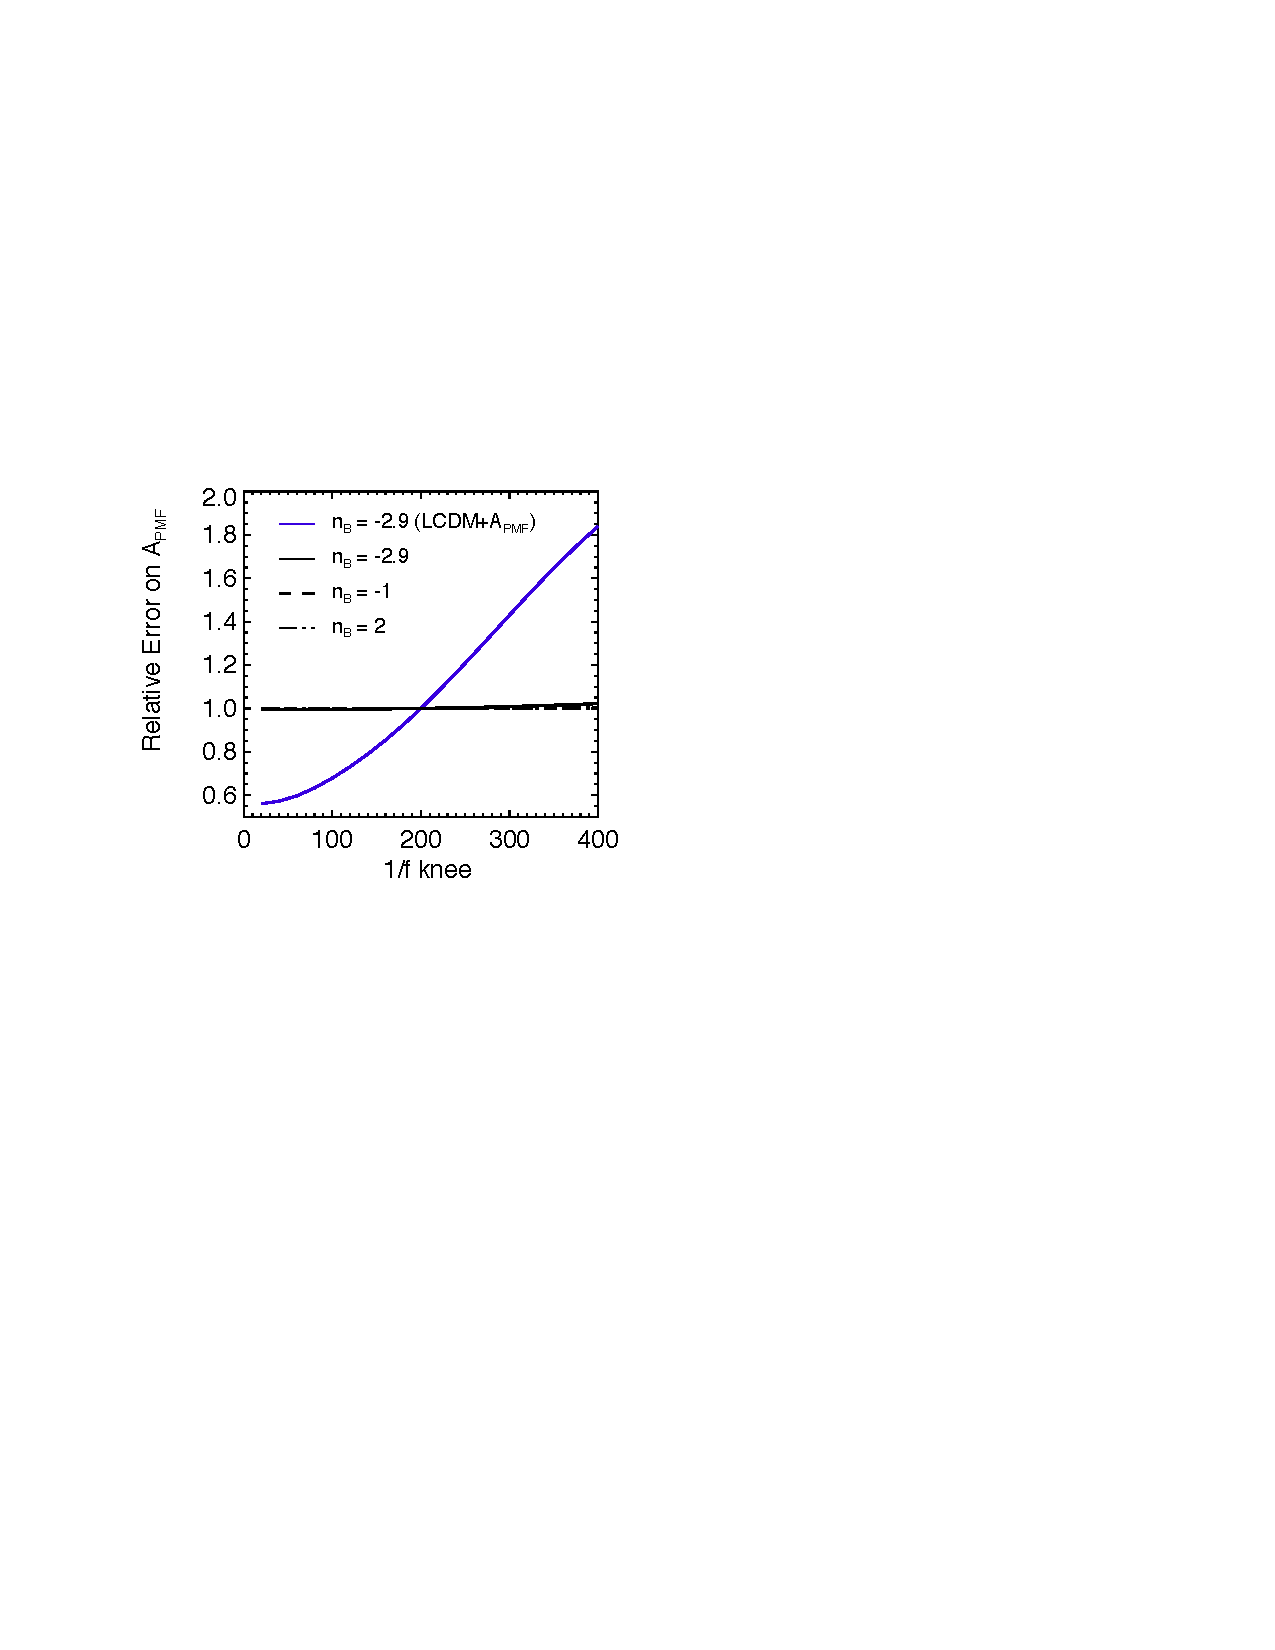
\includegraphics[width=0.9\textwidth,clip,trim={1.5cm 12.5cm 11cm 7.5cm}]{pmf_knee.pdf}
  \caption[CMB polarization from PMFs]{
  Currently dummy plot.
  Will be plot of BB bandpowers and PMF template.
      \label{fig:pmf-bb}
  }
\end{figure*}
 
\section{Results}
\label{sec:results}

We find the addition of ground-based CMB polarization data to \planck{} data substantially improves the upper limits on the allowed power due to a PMF, leading to a factor of two improvement. 
With Planck alone, the 95\% confidence upper limit is $\apmf <  0.68$ when $\alens$ is allowed to vary; with the ground-based experiments, this limit drops to $\apmf <  0.33$. 
We test which datasets are important by adding single datasets to the \planck{} set, and find that the majority of this improvement is due to the \bicepkeck{} ($\apmf <  0.36$) and \sptpol{} ($\apmf <  0.42$) B-mode power spectrum measurements. 
The other datasets do not have a large impact on the observed limits. 

We propagate these limits on the observed PMF power into limits on the magnetic field strength, \bpmf. 
Due to the scaling with the fourth power, an upper limit with a flat prior on \apmf{} would lead to an apparent `detection' of \bpmf. 
We therefor importance sample the chains to generate a flat prior on \bpmf. 
We find a 95\% limit of $\bpmf < XX$\,nG for \planck{} alone, consistent with \citep{planck15-19} with $n$ held fixed as we've done. 
This is reduced to $\bpmf < XX$\,nG for the combined dataset. 











\begin{table*}[h]
\begin{center}
\caption{\label{tab:param_all} All parameter constraints}
\tiny
\begin{tabular}{l || c c c c c c c | c}
Chain & $\Omega_b h^2$  & $\Omega_c h^2$  & $\theta$  & $\tau$  & logA  & $n_s$  & $A_{lens}$  & $A_{pmf}$ \\
lcdm\_alens\_all & $ 0.02240\pm  0.00026$ & $ 0.1179\pm  0.0020$ & $ 1.04106\pm  0.00047$ & $ 0.064\pm  0.016$ & $ 3.057\pm  0.030$ & $ 0.9696\pm  0.0062$ & $ 1.121 \pm  0.064$ & $< 0.33$ \\
lcdm\_alens\_nopmf\_all & $ 0.02241\pm  0.00024$ & $ 0.1179\pm  0.0020$ & $ 1.04106\pm  0.00047$ & $ 0.065\pm  0.016$ & $ 3.059\pm  0.029$ & $ 0.9694\pm  0.0062$ & $ 1.136 \pm  0.063$ & $< 0.00$ \\
lcdm\_alens\_nopmf\_planck & $ 0.02256\pm  0.00027$ & $ 0.1173\pm  0.0021$ & $ 1.04121\pm  0.00048$ & $ 0.069\pm  0.017$ & $ 3.067\pm  0.030$ & $ 0.9721\pm  0.0063$ & $ 1.175 \pm  0.067$ & $< 0.00$ \\
lcdm\_alens\_planckTT & $ 0.02252\pm  0.00031$ & $ 0.1174\pm  0.0027$ & $ 1.04122\pm  0.00053$ & $ 0.070\pm  0.050$ & $ 3.068\pm  0.098$ & $ 0.9713\pm  0.0080$ & $ 1.155 \pm  0.136$ & $< 1.34$ \\
lcdm\_alens\_planckTT\_TEB & $ 0.02264\pm  0.00029$ & $ 0.1161\pm  0.0025$ & $ 1.04141\pm  0.00053$ & $ 0.055\pm  0.021$ & $ 3.036\pm  0.042$ & $ 0.9755\pm  0.0072$ & $ 1.241 \pm  0.104$ & $< 0.77$ \\
lcdm\_alens\_planck & $ 0.02254\pm  0.00026$ & $ 0.1173\pm  0.0020$ & $ 1.04121\pm  0.00046$ & $ 0.068\pm  0.016$ & $ 3.065\pm  0.030$ & $ 0.9723\pm  0.0062$ & $ 1.171 \pm  0.070$ & $< 0.68$ \\
lcdm\_alens\_planck\_bicep & $ 0.02255\pm  0.00026$ & $ 0.1174\pm  0.0020$ & $ 1.04120\pm  0.00047$ & $ 0.069\pm  0.017$ & $ 3.067\pm  0.030$ & $ 0.9724\pm  0.0063$ & $ 1.177 \pm  0.068$ & $< 0.36$ \\
lcdm\_alens\_planck\_pb & $ 0.02255\pm  0.00027$ & $ 0.1173\pm  0.0021$ & $ 1.04119\pm  0.00046$ & $ 0.068\pm  0.017$ & $ 3.066\pm  0.031$ & $ 0.9725\pm  0.0064$ & $ 1.171 \pm  0.068$ & $< 0.63$ \\
lcdm\_alens\_planck\_sptpolB & $ 0.02254\pm  0.00026$ & $ 0.1173\pm  0.0020$ & $ 1.04121\pm  0.00047$ & $ 0.069\pm  0.017$ & $ 3.067\pm  0.030$ & $ 0.9724\pm  0.0062$ & $ 1.159 \pm  0.067$ & $< 0.42$ \\
lcdm\_alens\_planck\_sptpolE & $ 0.02239\pm  0.00025$ & $ 0.1178\pm  0.0020$ & $ 1.04107\pm  0.00048$ & $ 0.064\pm  0.016$ & $ 3.057\pm  0.030$ & $ 0.9698\pm  0.0061$ & $ 1.119 \pm  0.067$ & $< 0.73$ \\
lcdm\_planck & $ 0.02225\pm  0.00023$ & $ 0.1184\pm  0.0020$ & $ 1.04102\pm  0.00047$ & $ 0.066\pm  0.017$ & $ 3.062\pm  0.030$ & $ 0.9682\pm  0.0060$ & $ 0.000 \pm  0.000$ & $< 0.73$ \\
lcdm\_r\_alens\_all & $ 0.02240\pm  0.00025$ & $ 0.1178\pm  0.0020$ & $ 1.04107\pm  0.00046$ & $ 0.064\pm  0.016$ & $ 3.056\pm  0.029$ & $ 0.9702\pm  0.0062$ & $ 1.123 \pm  0.063$ & $< 0.27$ \\
\end{tabular}
\tablecomments{ 
Summary of results (will be trimmed for paper). 
} \normalsize
\end{center}
\end{table*}


\begin{table*}[h]
\begin{center}
\caption{\label{tab:param_all2} All parameter constraints2}
\tiny
\begin{tabular}{l || c c c c c c c | c}
Chain & $\Omega_b h^2$  & $\Omega_c h^2$  & $\theta$  & $\tau$  & logA  & $n_s$  & $A_{lens}$  & $A_{pmf}$ \\
lcdm\_alens\_all\_bk14 & $ 0.02240\pm  0.00025$ & $ 0.1179\pm  0.0020$ & $ 1.04106\pm  0.00045$ & $ 0.065\pm  0.017$ & $ 3.058\pm  0.030$ & $ 0.9696\pm  0.0060$ & $ 1.131 \pm  0.061$ & $< 0.27$ \\
lcdm\_alens\_all\_bk14\_tensor & $ 0.02243\pm  0.00025$ & $ 0.1178\pm  0.0020$ & $ 1.04110\pm  0.00047$ & $ 0.066\pm  0.017$ & $ 3.060\pm  0.030$ & $ 0.9704\pm  0.0062$ & $ 1.142 \pm  0.060$ & $< 0.29$ \\
lcdm\_alens\_all\_bk14\_vector & $ 0.02240\pm  0.00025$ & $ 0.1181\pm  0.0019$ & $ 1.04107\pm  0.00046$ & $ 0.064\pm  0.016$ & $ 3.056\pm  0.029$ & $ 0.9687\pm  0.0061$ & $ 1.134 \pm  0.061$ & $< 0.68$ \\
lcdm\_alens\_nopmf\_all\_bk14 & $ 0.02244\pm  0.00025$ & $ 0.1179\pm  0.0020$ & $ 1.04109\pm  0.00046$ & $ 0.066\pm  0.016$ & $ 3.061\pm  0.029$ & $ 0.9700\pm  0.0060$ & $ 1.145 \pm  0.061$ & $< 0.00$ \\
lcdm\_alens\_planck\_bk14 & $ 0.02256\pm  0.00027$ & $ 0.1174\pm  0.0020$ & $ 1.04120\pm  0.00048$ & $ 0.069\pm  0.017$ & $ 3.068\pm  0.030$ & $ 0.9723\pm  0.0062$ & $ 1.188 \pm  0.066$ & $< 0.28$ \\
lcdm\_alens\_planck\_bk14\_tensor & $ 0.02257\pm  0.00026$ & $ 0.1173\pm  0.0020$ & $ 1.04121\pm  0.00047$ & $ 0.069\pm  0.017$ & $ 3.067\pm  0.030$ & $ 0.9727\pm  0.0060$ & $ 1.186 \pm  0.065$ & $< 0.29$ \\
lcdm\_alens\_planck\_bk14\_vector & $ 0.02241\pm  0.00029$ & $ 0.1180\pm  0.0021$ & $ 1.04114\pm  0.00048$ & $ 0.065\pm  0.017$ & $ 3.058\pm  0.030$ & $ 0.9670\pm  0.0074$ & $ 1.149 \pm  0.075$ & $< 4.64$ \\
lcdm\_all\_bk14 & $ 0.02223\pm  0.00021$ & $ 0.1182\pm  0.0018$ & $ 1.04113\pm  0.00049$ & $ 0.074\pm  0.014$ & $ 3.074\pm  0.024$ & $ 0.9686\pm  0.0055$ & $ 0.000 \pm  0.000$ & $< 0.35$ \\
lcdm\_all\_bk14\_tensor & $ 0.02220\pm  0.00024$ & $ 0.1186\pm  0.0019$ & $ 1.04100\pm  0.00047$ & $ 0.067\pm  0.016$ & $ 3.063\pm  0.029$ & $ 0.9672\pm  0.0057$ & $ 0.000 \pm  0.000$ & $< 0.31$ \\
lcdm\_all\_bk14\_vector & $ 0.02215\pm  0.00022$ & $ 0.1188\pm  0.0020$ & $ 1.04088\pm  0.00046$ & $ 0.064\pm  0.016$ & $ 3.056\pm  0.028$ & $ 0.9653\pm  0.0055$ & $ 0.000 \pm  0.000$ & $< 0.83$ \\
lcdm\_r\_alens\_all\_bk14 & $ 0.02242\pm  0.00025$ & $ 0.1175\pm  0.0021$ & $ 1.04111\pm  0.00048$ & $ 0.068\pm  0.018$ & $ 3.063\pm  0.032$ & $ 0.9710\pm  0.0063$ & $ 1.133 \pm  0.062$ & $< 0.24$ \\
\end{tabular}
\tablecomments{ 
Summary of results (will be trimmed for paper). 
} \normalsize
\end{center}
\end{table*}


\section{Forecasts}
\label{sec:forecasts}

The sensitivity of CMB experiments is increasing rapidly due to the exponential growth in detector counts
\citet{s4sciencebook} thus defines four stages of CMB experiments. 
The current experiments (i.e.~the ones used for PMF constraints in the last section) are classified as Stage II experiments. 
Stage III experiments such as SPT-3G, the Simons Array, or AdvACTPol \citep{spt3g,simonsarray,advactpol} have approximately ten times more detectors, and generically will start collecting data in 2017 and finish in 2020-21.
In this section, we forecast the expected constraints from the Stage III experiments by combining forecasts for SPT-3G and the Simons Array. 
There is also a proposal to build a stage IV experiment, CMB-S4,  that would increase the detector counts by another order of magnitude and hopefully begin taking data in the early 2020s.
We examine the likely PMF constraints from CMB-S4, and consider which aspects of experimental or survey design are important to maximize the recovered information on PMFs.




\subsection{Methods and Experimental Parameters}

We use Fisher matrices to forecast the constraints on PMFs possible from each generation of experiment. 
Fisher matrices make it easy to combine different experiments and forecast the final parameter constraints \citep{fisher}. 
According to the Cramer-Rao bound, the Fisher information provides a lower bound on the uncertainty. 

We include two external datasets in all forecasts. 
The first dataset is the expected measurements of the  TT, TE and EE spectra from the \planck{} satellite. 
We include \planck{} TT information in the multipole range $2\le \ell \le 3000$. 
Due to the importance of galactic foreground removal at large scales in polarization, we only use TE and EE information starting from $\ell = 30$. 
A prior on the optical depth of 0.005 is added to account for the expected optical depth constraint from the missing multipoles. 
Second, we include a 1\% external measurement of the Hubble constant, such as would be expected from the Taipan experiment \citep{taipan}. 

One concern with combining Fisher matrices from different experiments is double-counting modes due to overlapping sky coverage. 
We sidestep this issue for the TT or TE spectra, by only using the \planck{} measurements. 
We do not expect the future experiments to substantially improve upon \planck{} in these spectra which are already cosmic variance limited out to fairly high multipoles. 
We throw away \planck{} EE data in the overlap region by appropriately increasing the forecasted \planck{} EE uncertainties. 
The exact increase depends on the assumed stage III or IV survey area.
We do not include \planck{} BB information in the forecasts. 
We ignore overlaps between the stage III  with the note that the overlap between a Chilean experiment like the Simons Array and South Pole experiment like SPT-3G should be small.
We do not include the stage III experiments, except as a prior on the polarized Poisson power, in the CMB-S4 constraints. 
With these measures, no modes should be double-counted in this analysis. 

\begin{table*}[h]
\begin{center}
\caption{\label{tab:experiments} Assumed survey parameters}
\small
\begin{tabular}{l || c c c c c }
Experiment & Sky coverage & Polarized Noise level  & 1/f knee & Beam FWHM \\
& &($\mu$K-arcmin)&&(arcmin.)\\
\hline
Stage III: & & & & \\

~~~~SPT-3G & 6\% & 3.0 & 200 & 1.2 \\
~~~~Simons Array & 36\% & 9.5 & 200 & 3.5 \\ 
\\
%\hline
CMB Stage IV & 55\% & 1.3 & 100 & 4.0 \\
\end{tabular}
\tablecomments{ 
Key numbers about the planned stage III and IV experiments. 
The sky coverage percentages are after galactic cuts. 
Unless otherwise noted,  the Fisher matrix forecasts in this work use these numbers. 
All forecasts also include beam and calibration uncertainty as noted in the text. 
} \normalsize
\end{center}
\end{table*}


We list the assumed survey areas, noise levels and beam sizes for each experiment in Table~\ref{tab:experiments}. 
We also assume a 5\% uncertainty on the beam FWHM and a 1\% power calibration uncertainty; we have tested relaxing or tightening the beam and calibration uncertainty and find these calibration terms have a negligible impact on the PMF constraints. 


We consider the constraints on PMFs in two cosmologies. 
In all cases, we also marginalize over unknown Poisson EE and BB  terms due to polarized extragalactic sources. 
Generally, we report constraints on the PMFs as one of several extensions to LCDM:  \lcdm{}  +r + \nrun{} + \neff{} + \mnu{}+ \apmf. 
However, in order to illustrate the degree to which parameter degeneracies are limiting the inferred constraints,  we also show constraints from an aggressive model in which the PMF power is the only extension to \lcdm{}:  \lcdm{}  + \apmf. 

As a sanity check, we look at the Fisher matrix forecasts for Planck alone as well in both of these cases. 
For both chains,  we look at the sigma in MCMC with \apmf{} allowed to go negative. 
While a negative \apmf{} is unphysical, this insulates the analysis against the data preferring negative values, and thereby producing tighter limits. 
We find for \lcdm{}  + \apmf{}: $\sigma(\apmf) = XX$ (to be compared to YY from the Fisher matrix). 
We find for the 11-parameter model: $\sigma(\apmf) = XX$ (to be compared to YY from the Fisher matrix). 
This degree of consistency is reasonable. \tbd{}

\subsection{Stage III forecasts}

The experiments that will begin taking data next year will dramatically improve constraints on the PMF power. 
With the minimal cosmological model, the 1-sigma forecasts for \planck{}+\ho{} is $\sigma(\apmf)=0.47$ as noted before.  
The uncertainty is forecast to fall nearly 400-fold by adding the two stage III experiments in this simplified model to $\sigma(\apmf)=0.0012$. 
Including all eleven parameters marginally weakens the \planck+\ho{} constraints on \apmf{} by 23\%, and the stage III constraint by a substantial factor of 2.5. 
Even so within this 11-parameter model, the addition of stage III CMB experiments improves the \apmf{} uncertainty by a factor of $\sim$\,180 to  $\sigma(\apmf)=0.0031$. 
We can expect substantially tighter constraints on PMFs by the end of the decade. 

\subsection{Stage IV forecasts}

The primary motivation behind the proposed CMB stage IV experiment is to search for inflationary gravitational waves and neutrino masses, however, the experiment should also enable extremely sensitive searches for PMFs. 
We begin by making forecasts for the fiducial CMB-S4 configuration as laid out in Table~\ref{tab:experiments}. 



\subsection{Survey considerations for Stage IV}

Given that CMB-S4 is still being designed, it is worthwhile to consider how the design decisions might influence the final PMF constraints. 
We look at four aspects of the experiment design: the telescope size or beam FWHM, the low-$\ell$ noise performance (1/f knee), and the choice of survey area, and how well the beam size and calibration must be known. 
Of these four, we find that the low-$\ell$ noise performance and survey area are important to searches for PMFs 

Larger telescopes will allow CMB polarization to be measured on smaller angular scales, and should therefor always improve the PMF constraints. 
However, larger telescopes are also more expensive to build which means at fixed cost, they would necessitate less ambitious focal planes and lower instantaneous mapping speed. 
We find the gains due to resolution at fixed mapping speed to be negligible: a beam size of FWHM=1$^\prime$ yields only a 1\% better limit than a FWHM of 10$^\prime$. 
This illustrates how important the large angular scales are to the PMF limits. 
We very crudely approximated a cost-neutral setup with a noise level of 1.3 \ukarcmin{} for a FWHM of 4$^\prime$; a noise level of 2.9 \ukarcmin{} for a FWHM of 2$^\prime$; and a noise level of 4.1 \ukarcmin{} for a FWHM of 1$^\prime$. 
In this quasi-cost-neutral setup, there is a strong preference to go for more detectors over better angular resolution: the uncertainty was a factor of 2.5 times smaller in the coarse case over the FWHM=1$^\prime$ case. 
Raw sensitivity is more important than angular resolution to an experiment's ability to study PMFs.

\begin{figure}[htb]\centering
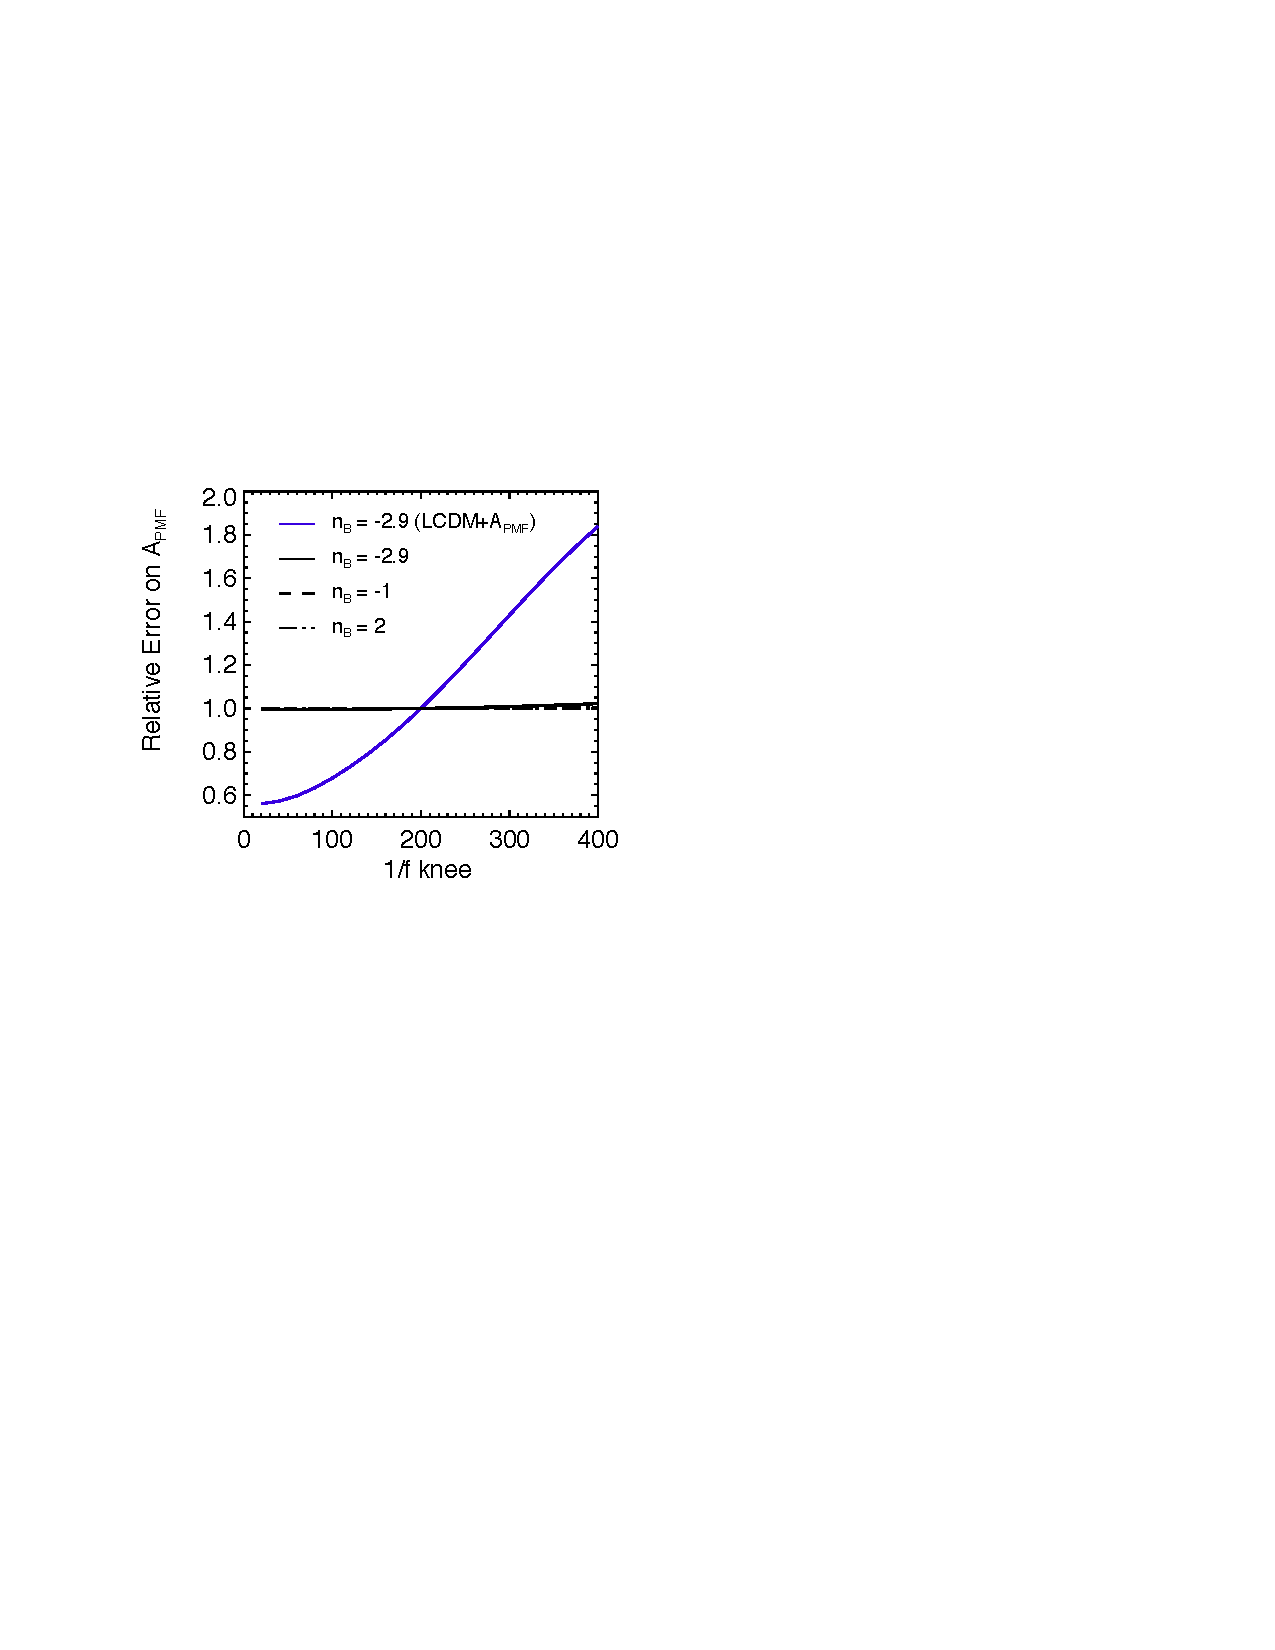
\includegraphics[width=0.45\textwidth,clip,trim={1.5cm 12.5cm 11cm 7.5cm}]{pmf_knee.pdf}
  \caption[Map knee dependence]{
  The forecasted uncertainty on the PMF power, \apmf{}, falls as expected as the low-frequency map noise decreases.  
  In particular, achieving a map 1/f knee frequency at or below $\ell = 200$ substantially improves the potential power of CMB-S4 PMF searches. 
  The black solid line shows the forecast uncertainty as a function of area in the 11-parameter cosmological model.
  The purple dot-dash line shows the same, except in the restricted \lcdm{}+\apmf{} 7-parameter model. 
  The x-axis is the map noise knee (see eqn.~\ref{eqn:knee}) in angular multipoles $\ell$. 
  As we expect, reducing low-frequency noise would lead to better PMF constraints. 
    \label{fig:knee}
  }
\end{figure}

Next we turn to the recovery of large angular scales, and the noise performance at low frequencies. 
We measure the importance by shifting the 1/f knee of the map-space noise in the range $\ell = [50,400]$. 
Effectively, we are multiplying the noise power, $N_\ell$, which is a constant for white noise,  by a function of angular multipole:
\be \label{eqn:knee}
f(\ell) = 1 + \left(\frac{\ell_{\rm knee}}{\ell}\right)^{8/3}.
\ee 
The exponent, 8/3, was selected based on a Kolmogorov spectrum of turbulence within a thin plane \citep{lay00}. %lay & halverson 2000. 
Note that this knob  serves as a placeholder for several effects, including a signal-to-noise hit due to galactic foregrounds or the methods used to clean these foregrounds, atmospheric noise, or actual instrumental 1/f noise. 
We find the results to be somewhat more sensitive to the 1/f knee in the simple \lcdm{}+\apmf{} model, where dropping \lknee{} from 400 to 50 reduces the uncertainty by a factor of 6.3.
However, the knee frequency is still important in the more conservative 11-parameter model, where the same shift reduces the uncertainties by a factor of 2.7. 
In both cases, as can be seen in Fig.~\ref{fig:knee}, the information loss really accelerates when the 1/f knee goes above $\ell \simeq 200$. 
For the same 11-parameter model, bringing \lknee{} to 200 from 400 yields a factor of 2 (only modestly worse than the 2.7x improvement for \lknee=50). 
Recovering large angular scales is clearly important to PMF searches. 
This is consistent with the study of telescope size in the last paragraph - which found extending to smaller angular scales only helped slightly. 
It is also consistent with the current upper limits, which are dominated by the BICEP2/Keck Array data at low-$\ell$. 
Fortunately, these large angular scales are also crucial to searches for inflationary gravitational waves, so the needs of the PMF search are well-aligned with one of the key science drivers for CMB-S4.

\begin{figure}[htb]\centering
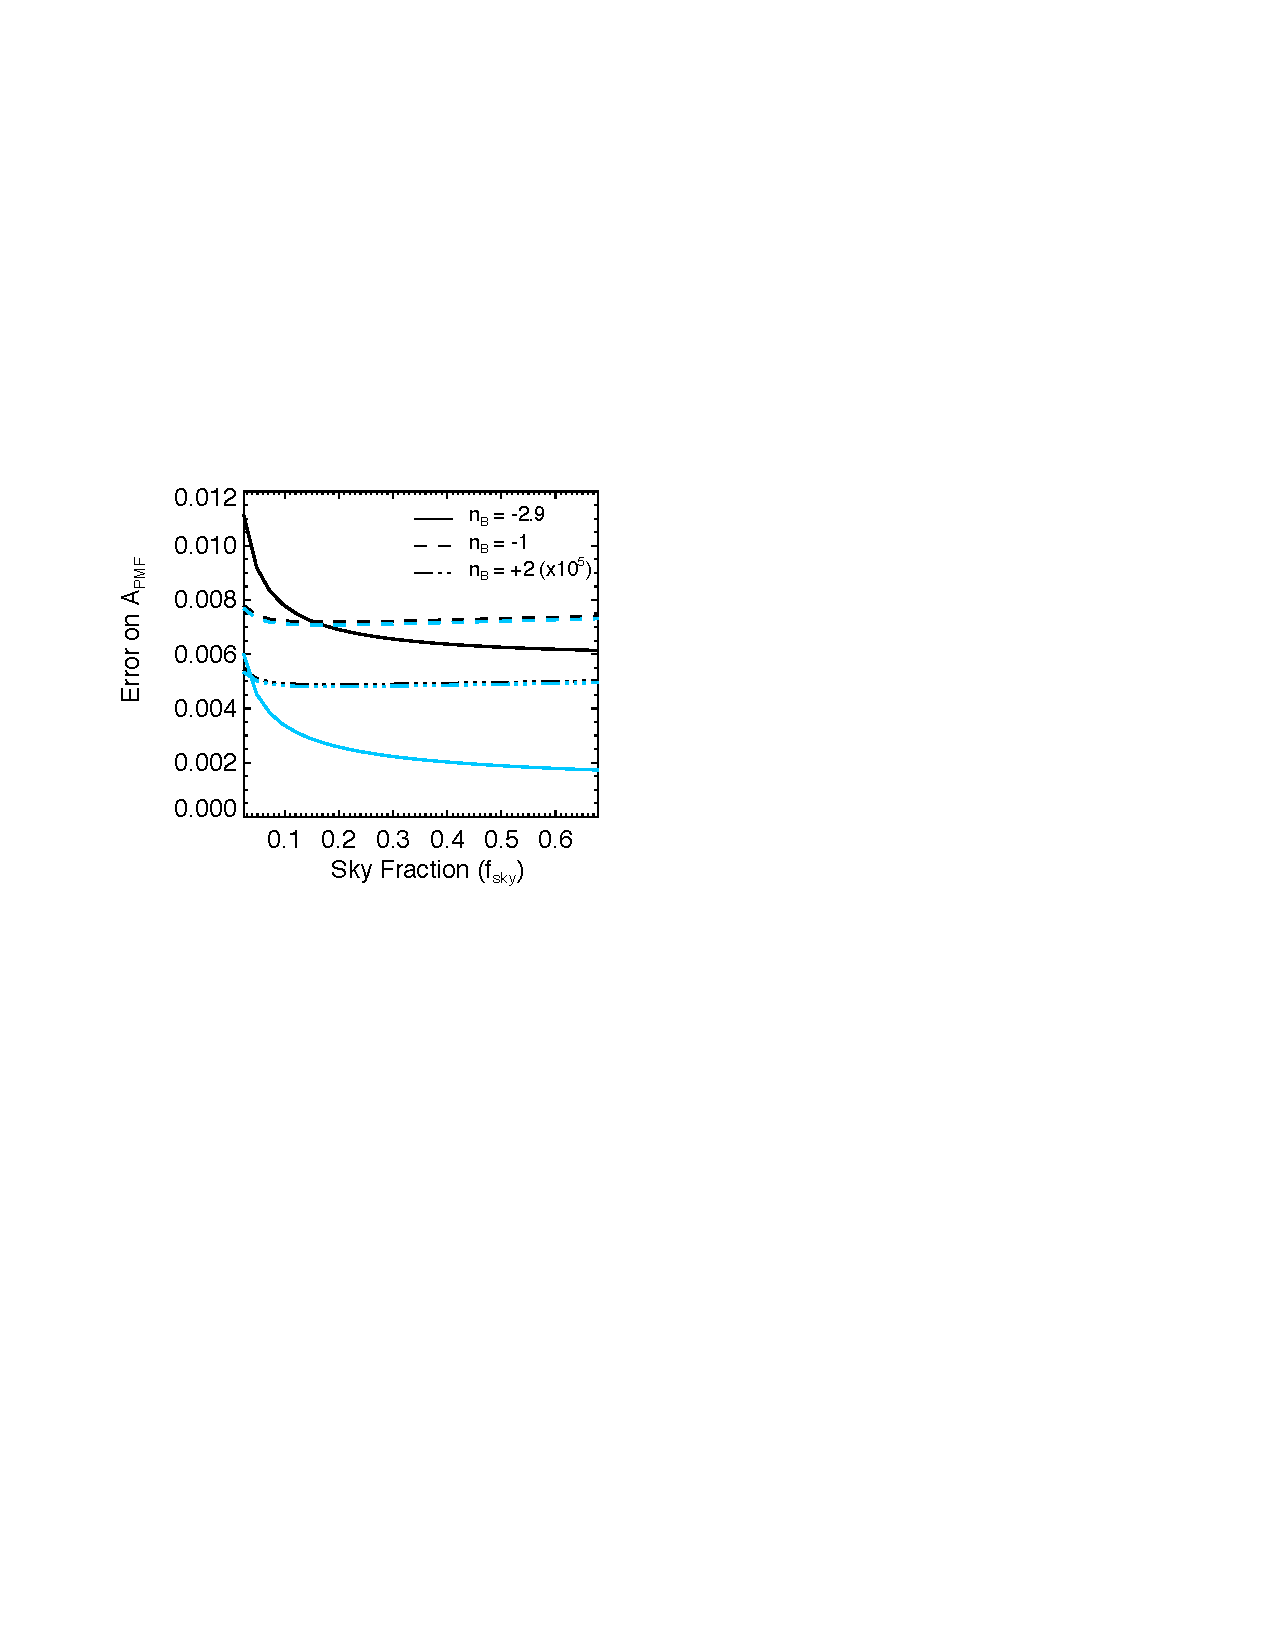
\includegraphics[width=0.45\textwidth,clip,trim={1.5cm 12.5cm 11cm 7.5cm}]{pmf_area.pdf}
  \caption[Area dependence]{
  The forecasted uncertainty on the PMF power, \apmf{}, falls as the survey area increases. 
  In particular, observing more than $\sim$\,15\% of the sky is strongly preferred for PMF searches. 
  The black solid line shows the forecast uncertainty as a function of area in the 11-parameter cosmological model.
  The purple dot-dash line shows the same, except in the restricted \lcdm{}+\apmf{} 7-parameter model. 
  In both cases, better limits on PMFs will be achieved with wider surveys.
    \label{fig:area}
  }
\end{figure}
A third question is whether it is better to integrate deeply on a small patch of sky or observe a wide area. 
As shown in  Fig.~\ref{fig:area}, it is better to go as wide as possible. 
A caveat to this analysis is that it is likely easier to remove galactic foregrounds to a specified level on targeted, `clean' patches as opposed to a substantial fraction of the sky, and we would expect galactic foregrounds to be important for the large angular scales. 
With that said, the PMF constraints improve by a factor of 1.4-1.5 (depending on the cosmological model) going from 10\% to 25\% of the full sky, and improve by another factor of 1.4-1.5 by going to the 70\% of the sky (the widest area likely to be possible after galactic cuts).


Finally, we consider if searches for PMFs introduce new requirements on the knowledge to which the instrumental beam or overall calibration of the experiments must be known. 
We parameterize the beam uncertainty as a fractional uncertainty on the FWHM of the Gaussian beam, and calibration uncertainty as an overall power uncertainty. 
We find negligible, sub-percent shifts in the forecasted uncertainty for calibration uncertainties from 0.2 to 5\% and beam FWHM uncertainties from 2 to 12.5\%. 
The PMF constraints are insensitive to beam and calibration uncertainty. 

\section{Conclusions}
\label{sec:conclusions}

In this work, we have improved the current upper limits on the strength of any primordial magnetic fields by including more CMB polarization data. 
By adding \bicepkeck{}, \pb, and \sptpol to \planck{} we find the 95\% CL upper limit on the PMF power falls from $\apmf < 0.68$ to $\apmf < 0.33$. 
The biggest contributor to this improvement is the low-$\ell$ data from \bicepkeck{}. 

We have also shown that the next generation of experiments have the potential power to dramatically reduce these limits, and potentially detect PMFs for the first time. 
The so-called stage III experiments, which should begin taking data in 2017, expect to set upper limits at the level of $\apmf < 0.0062$ even after marginalizing over a five-parameter extension to \lcdm.

The potential for detection increases even further with planned experiments like the Simons Observatory or CMB-S4. 
We show that an ideal version of CMB-S4 might decrease the 95\% CL upper limits eight-fold, to $\apmf < 0.0008$, and even non-ideal versions can easily set upper limits on order of $\apmf < 0.001$, i.e.~ a six-fold improvement over the forecasts for the stage III experiments and a 330-fold improvement over the current limits. 
These experiments will be very exciting probes of PMFs and other sources of cosmic birefringence. 

\bibliography{pmf}


\end{document}
